\section{Approach Overview}
\label{sec:approach-overview}

%\begin{figure*}[ht!]
 % \centering
  %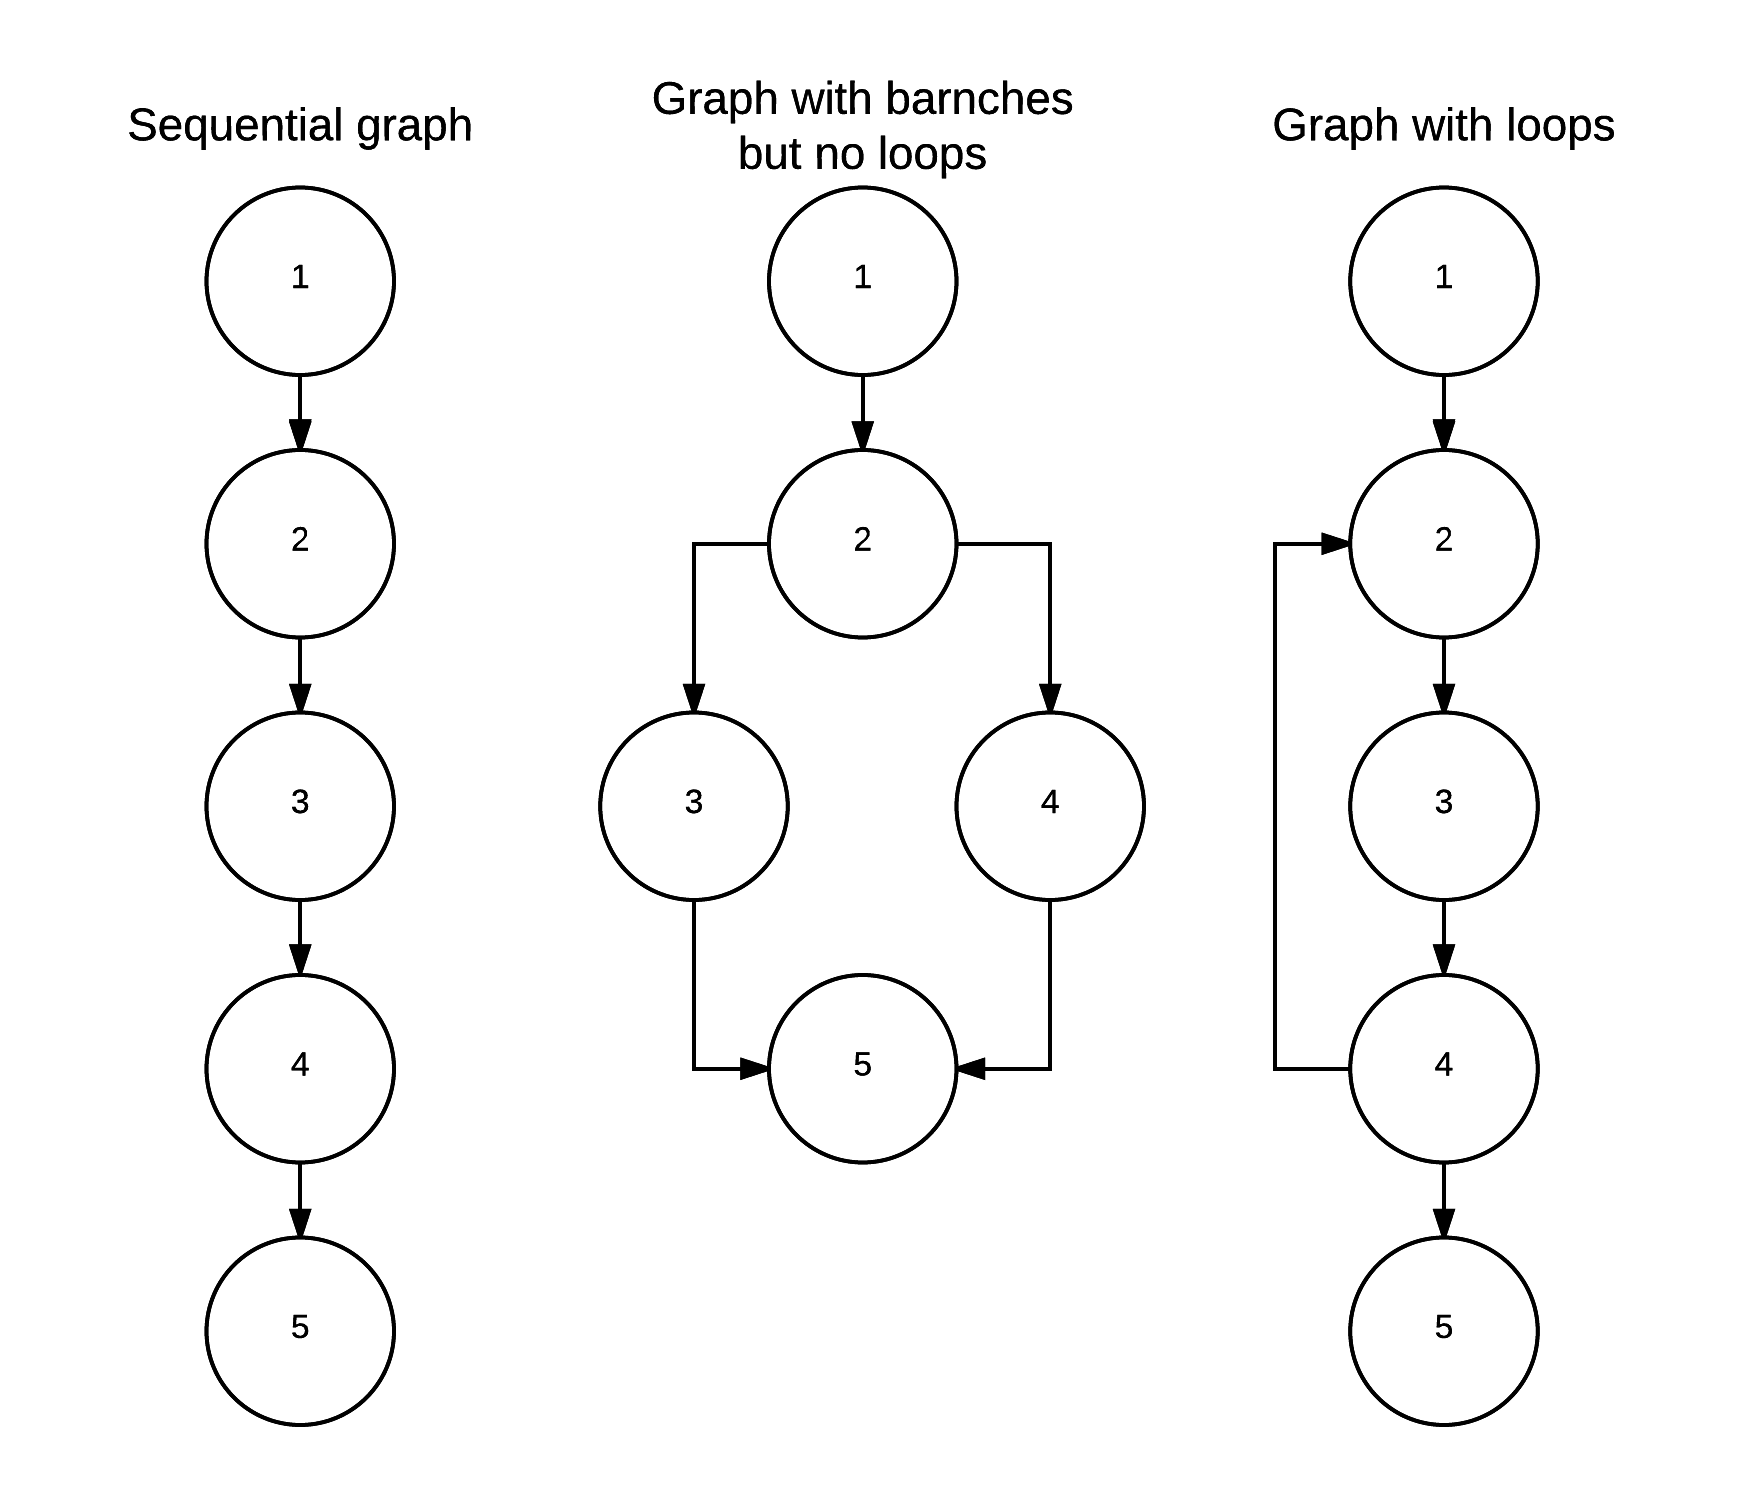
\includegraphics[width=0.54\linewidth]{tex-figures/graph.png}
%\caption{Example graphs.}
 % \label{fig:example-graph}
%\end{figure*}

\begin{figure*}[ht!]
  \centering
  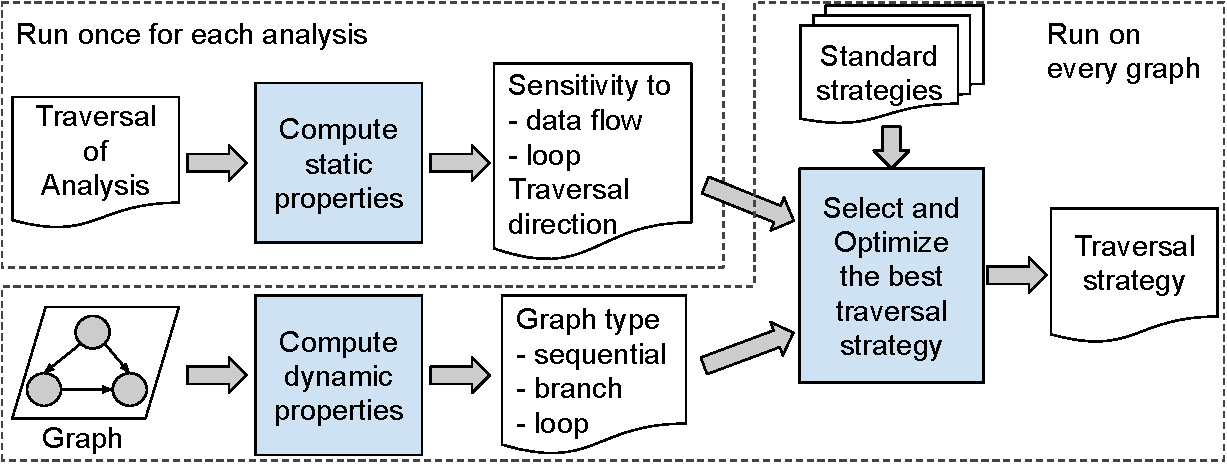
\includegraphics[width=\linewidth]{figures/overview.pdf}
\caption{Overview of the hybrid approach for selecting and optimizing graph traversal strategy.}
  \label{fig:overview}
\end{figure*}

Let us take the traverse operation in line 26 in the dominator analysis (Figure \ref{fig:dominator}) as our example traverse operation and a CFG with a loop and a branch \texttt{g} as our example CFG. The traverse operation applies the \texttt{dom\_T traversal} on \texttt{g} and is called with a fix-point \texttt{fp} with \texttt{FORWARD} traversal direction. We need to come up with the best traversal strategy to traverse \texttt{g} that completes the traverse operation faster than the other candidate traversal strategies. The overview of the hybrid approach for selecting and optimizing the graph traversal strategy is shown in Figure \ref{fig:overview}.

\subsection{Step 1 : Extract static properties from the traversal}
The first step is to analyze the traversal that is given as input in the traverse operation and extract the required static properties that we need, in-order to make the best traversal strategy decision. The required static properties are \textit{data flow sensitivity} of the traversal,% \textit{traversal sensitivity} of the traversal,% 
\textit{loop sensitivity} of the traversal and the \textit{traversal direction}.

%\begin{definition}
%\textbf{Traversal sensitivity} property is a property of the traversal that indicates whether the traversal is sensitive to the traversal strategy used to traverse the CFG and the result generated by the traversal at each node differs from one traversal strategy to another. If the traversal contains non commutative operations involving global variable, then such traversals are \textbf{traversal sensitive}.
%\end{definition} 
%\texttt{dom\_T} traversal in \textit{dominator analysis} does not contain any non commutative property involving global variable and hence it is determined as \textit{traversal in-sensitive}.
\begin{definition}
\textbf{Data flow sensitivity} property is a property of the traversal that indicates whether the traversal output of a node is dependent on the traversal output of other nodes. In line 13-14 of the dominator traversal, the \texttt{dom}
variable of current node n is dependent on the traversal output
of its predecessors. Hence \texttt{dom\_T} traversal in \textit{dominator analysis}
is data flow sensitive. Data flow sensitive traversal usually requires multiple traversal over the CFG untill all nodes reach fix-point ie the output of the nodes stabilizes.
\end{definition} 

\begin{definition}
\textbf{Loop sensitivity} property is a property of the data flow sensitive traversal that indicates whether the data flow in the traversal is affected by the loops present in the CFG. In data flow sensitive traversals, a node's output is dependent
on its neighbor's(successor/predecessor) output. If a back edge is present in the graph, then the back edge's destination
node will be visited before back edge's source node. Since the source node's output will not be available, the destination
node's output cannot be computed in the current traversal of the CFG
and hence another traversal is needed. Now we have to determine whether the traversal really needs the source node's
output to compute the destination node's output. From line 14 in \texttt{dom\_T} traversal, we can see that
\texttt{intersection} is used to merge the current node's traversal output with
its neighbor's traversal output. \texttt{Intersection} only shrinks a node's traversal output from one iteration to another. In this case, a back edge's
source node's traversal output can affect the back edge's destination
node's traversal output only if some element has been removed from the traversal output of
the source node, because only when an element is removed,
the set can further shrink in intersection and newly added elements does not affect in intersection operation. In \texttt{dom\_T} traversal of \textit{dominator analysis}, we can see that no element is removed from
the traversal output during the traversal and hence we can conclude that \texttt{dom\_T} traversal is \textit{loop insensitive}.
\end{definition}
Analysis direction is extracted from the traverse operation argument. In line 26 of the \texttt{dom\_T} traversal in \textit{dominator analysis}, we see that the analysis direction is \texttt{FORWARD}.
Hence we conclude that \texttt{dom\_T traversal} in \textit{dominator analysis} is \textit{%traversal in-sensitive,
	forward data flow sensitive and loop in-sensitive traversal}.

\subsection{Step 2 : Extract dynamic properties from the CFG}
The next step is to extract the required dynamic properties from the CFG \texttt{g}. The only property that is of interest to us is the type of control flow present in the CFG.
We classify CFGs into three types(\textit{Sequential CFG, CFG with branches and no loops, CFG with loops}) based on their control flow.
\begin{definition}
\textbf{Sequential CFG} are CFGs that does not have any branches or loops.
\end{definition}
\begin{definition}
\textbf{CFG with branches and no loops} are CFGs which have branches but no loops.
\end{definition}
\begin{definition}
\textbf{CFG with loops and no branches} are CFGs that has loops and do not contain any other branches.
\end{definition}
\begin{definition}
	\textbf{CFG with loops and branches} are CFGs that has loops and contains branches apart from the loops.
\end{definition}
Our input CFG \texttt{g} is a \textit{CFG with loops and branches}.

\subsection{Step 3 : Traversal strategy decision}
\begin{itemize}
%\item We first check whether our traversal is \textit{traversal sensitive} or not. If the traversal is sensitive to the traversal strategy used, the result of the traversals differs based on the used traversal strategy and hybrid approach cannot make decision for such traversals. Our example traversal, which is \texttt{dom\_T} traversal in \textit{dominator analysis} is \textit{traversal in-sensitive} and hence hybrid approach is applicable and we will choose the best traversal strategy that will finish the analysis faster.
\item The first step is to check whether our traversal is \textit{data flow sensitive} or not. We check this property because \textit{data flow sensitive} traversal requires multiple traversals over the CFG and hence we will try to choose the traversal strategy that visits lesser number of nodes and also does lesser number of operations per node. 
%\textit{Data flow in-sensitive} analysis requires single traversal of the CFG and hence we will choose the traversal strategy that does lesser number of operations per node. 
We have determined that \texttt{dom\_T} traversal is \textit{data flow sensitive}. In these kind of traversal, where traversal output at one node is dependent on traversal output of other nodes, a simple way to perform these traversal is to set up flow equations for each node of the CFG and solve them by repeatedly calculating the output from the input at each node until all the nodes reaches a fix-point. In order for all the nodes to reach fix-point, it may require multiple traversals over the CFG which is determined by the CFG structure.
\item We have determined that our CFG \texttt{g} contains loops. For CFGs containing loops, no traversal strategy can give a ordering of nodes that could solve the data flow sensitive traversal in a single traversal of the CFG. We now have to investigate whether the loop present in \texttt{g} affects the number of traversals in our data flow sensitive traversal.
\item We have determined that \texttt{dom\_T} traversal is \textit{loop in-sensitive} and therefore the loops present in \texttt{g} is not going to affect the data flow. We now investigate whether \texttt{g} contains any branches apart from the loops present. Our CFG does contain a branch. 
\item We then look at the \textit{traversal direction} and we have determined it to be \texttt{FORWARD}. For \textit{forward data flow sensitive} traversal, a traversal strategy can complete it in one traversal of the CFG only if the nodes are visited in such a way that each node is visited only after the node's predecessors. \textit{Reverse post-order} traversal guarantees such ordering of  nodes when CFG contains only branches. Though our CFG contains loop, we can ignore the loop present in our CFG as it does not affect the data flow. Without the loop, our CFG contains only branches and hence \textit{Reverse post-order} traversal will be chosen as the traversal strategy as it provides us with an ordering of nodes such that the analysis will reach fix-point in single traversal of the CFG.
%\item So for this CFG \texttt{g} and traversal \texttt{dom\_T}, the best traversal strategy is to visit the nodes in the increasing order of node ids since the node ids are assigned in a topological order. Traversing a sequential CFG in increasing topological order makes sure that a node is visited after its predecessors and hence we will complete the \texttt{dom\_T} traversal in a single traversal of the CFG. 
\item The next step is to optimize the chosen traversal strategy. We do not need fix-point checking operation to be done, as we knew from the static and dynamic properties that the traversal will be completed in single traversal and we do not need to check fix-point for each node to confirm. Hence we optimize the chosen traversal strategy to remove fix-point checking operation. Hence we visited the minimum number of nodes and also reduced the number of operations per node.
\end{itemize}
This is only one path to the traversal strategy decision in the decision tree and there exists many other paths which is shown in Figure \ref{fig:decision-tree}. The next section lists the candidate traversal strategies and explains our approach and the decision tree.